%%%%%%%%%%%%%%%%%%%%%%%%%%%%%%%%%%%%%%%%%%%%%%%%%%%%%%%%%%%%%%%%%%%%%%%%%%%%%%%%%%%%%%%%%%%%%
%%									Chapitre 4												%
%%%%%%%%%%%%%%%%%%%%%%%%%%%%%%%%%%%%%%%%%%%%%%%%%%%%%%%%%%%%%%%%%%%%%%%%%%%%%%%%%%%%%%%%%%%%%

\chapter{Imagerie dynamique de la circulation intracrânienne}
	\minitoc


%%%%%%%%%%%%%%%%%%%%%%%%%%%%%%%%%%%%%%%%%%%%%%%%%%%%%%%%%%%%%%%%%%%%%%%%%%%%%%%%%%%%%%%%%%%%%

Dans ce chapitre, nous allons faire la revue des données dynamiques qui nourriront notre modèle
biophysique. Nous commençons par un rappel des éléments physiologiques bien établis de la
circulation intracrânienne nous passons ensuite en revue les modalités d’imageries qui permettent
d’accéder au débit sanguin à différents niveaux dans le cerveau.
%%%
%%%
%%%
\section{Rappels sur la dynamique des écoulements intracrâniens}
%%%
%%%
\subsection{Artères, artérioles et autorégulation}
Le compartiment artériolaire représente le site primaire de la résistance vasculaire, il va être
en mesure de s’adapter pour répondre aux conditions physiologiques. En présence d’un tube rigide,
une corrélation forte existe entre le débit sanguin et la pression artérielle. Lorsque la pression
augmente, le diamètre du tube augmente par action mécanique du fait son élasticité et donc le flux
aussi. Mais le cerveau présente un mécanisme dit d’autorégulation capable d’agir comme un tampon
ajustant le diamètre des artérioles en réponse aux variations de pression et assurant un apport
constant et suffisant de ressources.
		
Une première autorégulation, dite métabolique, intervient en réponse au changement de
pression artérielle en $CO_2$ ($paCO_2$). Elle va réguler le débit sanguin cérébral en fonction des besoins du
tissu. L’autorégulation métabolique produit une vasodilatation pour augmenter le débit lorsque le pH
chute durant les évènements hypoxiques. Inversement, en phase d’hyperventilation, le pH augmente,
induisant une vasoconstriction et ainsi une diminution du volume sanguin cérébral (\cite{Hajjar2010}). La diminution
de pH entraine l’ouverture de canaux potassiques générant une hyperpolarisation de la cellule. Le
courant est transmis aux cellules musculaires lisses par des jonctions myoendothéliales ce qui ferme
les canaux calcium, baisse le calcium intracellulaire et ainsi relaxe les SMC.

Une seconde autorégulation intervient en réponse aux variations de pression. En effet le débit
sanguin cérébral est maintenu entre 50 et 60 mL/100g/min pour des pressions perfusionnelles cérébrales (CPP) de 60 à 160 mmHg. Cela traduit la présence d’un mécanisme d’autorégulation du
débit (Figure~\ref{fig:3_1_autoregulation}). Notons qu'à partir d'ici, le terme pression évoquera uniquement les pressions artérielles ou perfusionnelles selon les compartiments.

%%%
\begin{figure}[!t]
\centering
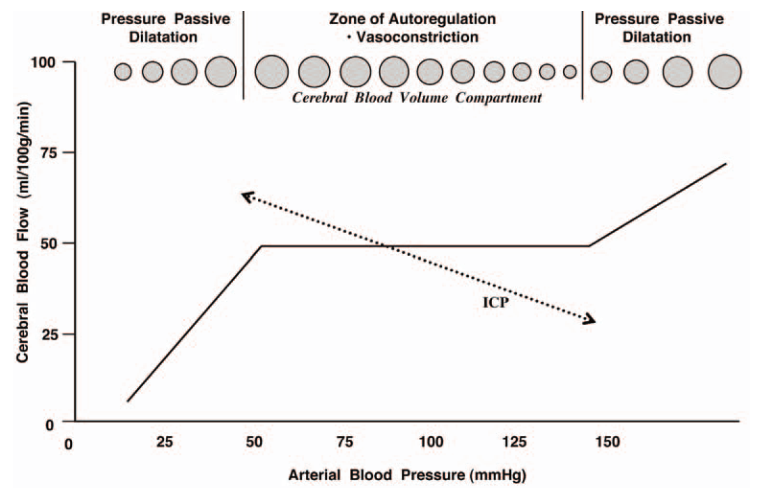
\includegraphics[width=14cm]{3_1_autoregulation}
\caption{Autorégulation du débit en fonction de la pression. Illustration de ~\cite{Lang2003}.}
\label{fig:3_1_autoregulation}	
\end{figure}
En dessous de pressions perfusionnelles de l’ordre de 60 mmHg, l’autorégulation est perdue
entrainant une ischémie. Le volume intracrânien étant constant, la perfusion doit s’adapter (\cite{Cipolla2009}). Pour
maintenir ce débit, le calibre des vaisseaux doit être ajusté. En cas de faible pression, le vaisseau est
dilaté (par un effet contraire à la mécanique), ce qui augmente le volume sanguin cérébral et donc la
pression intracrânienne. En haute pression, le vaisseau se contracte ce qui baisse le volume sanguin
cérébral et donc la pression intracrânienne (\cite{Lang2003}). Les mécanismes sous-jacents sont liés à une réponse
myogénique et une innervation sympathique qui limitent l’augmentation du débit sanguin cérébral. La
réponse myogénique est la capacité intrinsèque des cellules musculaires lisses à répondre aux
changements de charges mécaniques ou de pression intravasculaire. Le mécanisme de contraction et
dilatation en réponse à la pression est appelé effet de Bayliss (\cite{Cipolla2009}). Il est lié à une augmentation du
calcium intracellulaire qui augmente la phosphorylation des chaines légères de myosine et donc
génère une vasoconstriction. Un mécanisme de rétrocontrôle appelé « Calcium sparks » est présent
afin de contrôler cet effet.

Enfin une autorégulation dite neuro-astrocytaire existe, via des neurones qui se projettent
jusqu’aux vaisseaux corticaux et libèrent des neurotransmetteurs qui stimulent des récepteurs sur les
cellules musculaires lisses, l’endothélium ou les astrocytes ce qui induit une dilatation ou contraction
de concert avec la demande neuronale (\cite{Cipolla2009}).

La regulation du debit sanguin dans le cerveau est un mécanisme complexe assuré par les
artérioles permettant l’adaptation à des conditions execeptionnelles (modifications de pression,
hypoxie), tout en assurant un apport constant et adapté aux tissus (besoins métaboliques).
%%%
%%%
\subsection{Microcirculation}
Le lit capillaire du cerveau est constitué d’un réseau dense de vaisseaux inter communicants
bordées de cellules endothéliales mais ne disposant pas de cellules musculaires lisses (\cite{Rennels1975}), ils ne
peuvent donc pas participer à la régulation du débit. La longueur totale des capillaires dans le cerveau
humain est de 640 km (\cite{Abbott2010}). C’est le site principal de l’échange d’oxygène et de nutriments. Cet échange
est bien sur dépendant de la longueur du trajet et du temps de transit des globules rouges. Dans le
cerveau, tous les capillaires sont perfusés à tout moment, et il a été estimé que presque chaque
neurone dans le cerveau a son propre capillaire (\cite{Zlokovic2005}). Cela met en évidence la relation critique qui existe
entre le compartiment neuronal et vasculaire. Le gradient de pression intravasculaire entre les
artérioles précapillaires et les veinules postcapillaires est le régulateur principal du flux capillaire. La
régulation du débit dans la microcirculation est donc dépendante de la régulation du flux et de la
pression micro vasculaire dans les artérioles. La vitesse des globules rouge dans les capillaires cérébraux est élevée (~1 mm/sec) et hétérogène (de 0.3 à 3.2 mm/sec) (\cite{Wei1993}). L’hétérogénéité des
vitesses des flux est importante pour le transport effectif de l’oxygène au tissu neuronal dont la
demande métabolique fluctue régulièrement vers des valeurs considérables.

En conditions normales, la densité des capillaires varie significativement dans le cerveau en
fonction de la localisation et de l’énergie requise. La densité est naturellement plus grande dans la
matière grise en comparaison de la matière blanche (\cite{Klein1986}). Les états pathologiques, physiologiques, et
environnementaux peuvent influencer ou promouvoir les changements de densité des capillaires.
Celle-ci peut doubler après une à 3 semaines d’hypoxie chronique. Cette augmentation adaptative
augmente le volume sanguin cérébral et restore la tension des tissus en oxygène (\cite{Cipolla2009}). L’hypertension
affecte elle aussi la densité, elle cause une raréfaction des capillaires et affaiblit la formation des
microvaisseaux ce qui augmente la résistance vasculaire.

%%%
%%%
\subsection{Veines }
Le système veineux cérébral est constitué de veines n’ayant pas de propriétés de régulation et
soumises par conséquent à des vagues de pression venant de la pulsation des artères en amont. Le
flux artériel systolique cérébral est en effet couramment considéré comme la force motrice qui met en
mouvement tous les fluides intracérébraux. En particulier, c’est lui qui entraîne la ventilation veineuse
durant la systole (\cite{Greitz1992}). Physiologiquement, le système veineux est donc considéré comme
principalement passif et influencé par des facteurs extravasculaires. La configuration anatomique des
veines confirme cette conception puisqu’elle diffère de celle des artères, du fait qu’elles ne disposent
pas de couches de muscles lisses et donc ne peuvent faire varier leur lumière activement. La pression
dans le flux veineux est estimée à 20 ± 5 mmHg dans les veines sous arachnoïdes (\cite{Ekstedt1978}) et est le résultat
du bilan de la pression résiduelle capillaire, de la pression intracrânienne et des pressions en aval dans
le sinus veineux. Bien que les valeurs de pressions des artères soient hautement atténuées lorsqu’elles
franchissent le lit capillaire et atteignent le système veineux, les pulsations de la pression
intracrânienne se traduisent par une pulsation de la pression veineuse intracrânienne (\cite{Elsankari2012}).

%%%
%%%
\subsection{Le liquide céphalo-rachidien}
Le liquide céphalo rachidien ou liquide cérébro-spinal (LCS) est un milieu régulateur pour le
cerveau, sur le plan mécanique et sur le plan biochimique. Sa composition et son volume sont
maintenus constant. Il joue le rôle de milieu intérieur du système nerveux central. Il existe des
échanges permanents entre le LCS profond intra-ventriculaire et le LCS des espaces sous
arachnoïdiens. Le LCS présente donc un mouvement lent et global qui l’entraîne de son lieu de
production à son lieu de résorption. C’est donc l’équilibre en sécrétion et résorption qui assure chez le
sujet normal la constance du volume du LCS.

Le LCS est sécrété par les plexus choroïdes (80\%) et des structures extra-plexuelle telles que le
revêtement épendymaire des ventricules, les espaces sous arachnoïdiens intracrâniens et les espaces
sous arachnoïdiens spinaux (20\%). La production est réalisée à partir du plasma sanguin selon un
mécanisme actif de filtration et de sécrétion avec un taux de 500 ml/24h (renouvellement 3 à 4 fois
par jour) (\cite{Maurer2010}).

%%%
\begin{figure}[!t]
\centering
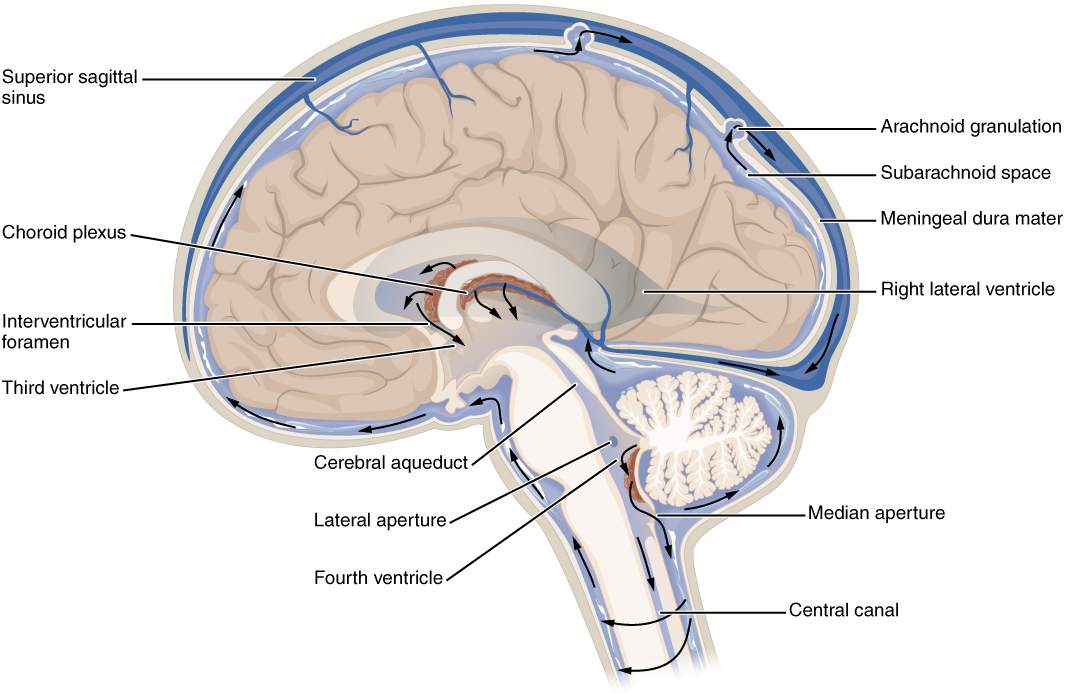
\includegraphics[width=14cm]{3_2_LCR}
\caption{Circulation du LCS.}
\label{fig:3_2_LCR}	
\end{figure}
Différents sites de résorption et différents mécanismes assurent la résorption du LCS (Figure~\ref{fig:3_2_LCR}) au niveau des villosités arachnoïdiennes invaginées dans le sinus veineux dure-mériens, en
particulier le sinus sagittal supérieur (\cite{Segal2001}). Le mécanisme est lié à la pression hydrostatique et à la
différence de pression osmotique entre le LCS et le plasma : une pression importante du LCS génère
un flux sortant qui est au contraire stoppé par une pression veineuse importante. D’autres structures participent à la résorption, telles que les granulations de Pacchioni ou les plexus choroïdes et le
système lymphatique qui permet un drainage complémentaire.

Le LCS des ventricules latéraux circule par le trou de Monro vers le troisième ventricule. Du
troisième ventricule, il circule ensuite par l’étroit aqueduc cérébral vers le quatrième ventricule. Il
quitte alors le système ventriculaire et entre dans les citernes (espaces élargis dans l’espace sous-
arachnoïde) par les trous de Luschka et de Magendie et dans l’espace sous-arachnoïde qui entoure
l’encéphale (\cite{Bernard2007}). Il est finalement réabsorbé dans le sang au niveau du sinus veineux par les
granulations arachnoïdiennes.
%%%
%%%
\subsection{Hypothèse de Monro-Kellie}
La contrainte principale qui gouverne l’hémodynamique intracrânienne est la constance stricte
du volume de cet espace. Selon les hypothèses de Monro-Kellie, la somme des volumes des différents
composants de la cavité intracrânienne (sang, cerveau, et LCS) reste toujours constante (\cite{Carmelo2002}). Ainsi, une
augmentation de l’un de ces paramètres doit engendrer une réduction de l’un ou des deux restants.
Le volume intracrânien est incompressible en conditions physiologiques, le sang circulant dans le crâne
est donc de volume constant à tout temps. La dilatation artérielle ne peut être réalisée que grâce à
une réduction des veines intracrâniennes qui peut être obtenu par diminution de la pression veineuse
(\cite{Wei1982}). Chaque augmentation de volume dans une partie de l’espace intracrânien requiert une
compensation.
%%%
%%%
%%%
\section{Imagerie de la dynamique}
On distinguera dans la circulation intracrânienne deux types de débits, tout d’abord le débit
macroscopique dans les principaux compartiments : système artériel, système veineux, liquide
cérébro-spinal. Par ailleurs, un débit de perfusion plus distal dans les lits capillaires. Les techniques
d’imagerie permettant d’accéder à ces deux dynamiques ne sont pas les mêmes. Nous allons dans un
premier temps voir comment recueillir des informations sur les débits macroscopiques avant
d’évoquer la perfusion.
%%%
%%%
\subsection{Débits macroscopiques : imagerie en contraste de phase en mode cinétique}
Nous avons vu lors des précédents paragraphes que l’imagerie de contraste de phase
permettait d’accéder à la structure des vaisseaux (artères et veines) en utilisant le déphasage des spins
mobiles soumis à un gradient bipolaire. Cet outil peut néanmoins permettre, et c’est son principal
intérêt, de quantifier les vitesses et débits dans les artères, les veines et le liquide cérébro-spinal avec maintenant des résolutions spatiales relativement fines (0.4 mm).

Ces acquisitions sont réalisées en 2D voir en 2D multicoupes (2 ou 3). Le plan de coupe doit être
perpendiculaire au vaisseau exploré et l’acquisition synchronisée sur le cycle cardiaque. Toutes les
images ne pouvant être acquises au cours d’un seul cycle cardiaque, l’acquisition est réalisée sur
plusieurs cycles, les images étant acquises à différents moments dans celui-ci.

Le décalage de phase $\Delta \phi$ mesuré est proportionnel à la vitesse du proton dans le vaisseau dans
la limite d’un angle de 2$\pi$, soit $\pm \pi$. Ainsi lorsque le décalage est supérieur à 2$\pi$ on peut observer des
repliements de phases ou saut de phase (voir~\ref{sec:QSM_chap_2}).

La présence de ce genre d’artéfacts traduit l’utilisation d’un gradient trop important en rapport
des vitesses attendues dans le vaisseau exploré. Afin d’éviter ce problème, le gradient doit être ajusté.
Il faut donc connaître l’ordre de grandeur de la vitesse maximale à mesurer et pour cela, une
présélection d’une échelle des vitesses permet d’optimiser le rapport signal sur bruit (RSB) et
d’améliorer la sensibilité de la technique. Le principe de cette présélection consiste à définir le
déphasage engendré par unité de vitesse. Ainsi, on définit la vitesse maximale codée $V_{enc}$ qui va
permettre de limiter ces artéfacts tout en conservant une bonne dynamique de la mesure. En effet,
placer $V_{enc}$ à une valeur trop grande en rapport des vitesses dans le vaisseau induirait un déphasage
très faible et donc une perte de la dynamique.

Si malgré tout quelques artefacts subsistent, il reste possible de les corriger simplement en
utilisant les algorithmes de dépliement au cours du temps (Figure~\ref{fig:3_3_depliement_phase}).
%%%
\begin{figure}[!t]
\centering
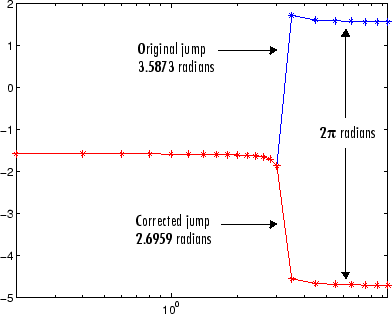
\includegraphics[width=9cm]{3_3_depliement_phase}
\caption{Exemple de dépliement de phase. En bleu la cinétique initiale du signal avec la présence d'un saut de
phase. En rouge la nouvelle cinétique après dépliement. Source : http://fr.mathworks.com}
\label{fig:3_3_depliement_phase}	
\end{figure}
Pour chaque pixel on peut par la suite extraire la vitesse en utilisant la formule sur la base du
déphasage $\Delta \phi$ observé :
\begin{equation}
v\,=\,\biggl(\frac{\Delta\phi}{\pi}\biggr)\,*\,V_{enc}.
\end{equation}
Ainsi, grâce à cette équation, il est possible d’estimer la vitesse (en cm/s) dans la direction du codage
de flux. En multipliant la vitesse par l’aire d’un pixel, on peut aussi estimer le débit (en mL/s). Cela
permet d’obtenir le débit à travers un vaisseau en multipliant la vitesse moyenne dans la zone d’intérêt
par l’aire de cette zone. On rappel que l'on suppose une accélération nulle.

La formule de base du contraste de phase est simple. La vitesse peut être calculée à partir du
déphasage et de la vitesse d’encodage. Or pour extraire la vitesse moyenne ou le débit au sein d’un
vaisseau, il convient de le segmenter au cours du temps, son diamètre évoluant avec le cycle cardiaque.
Le problème principal est la très grande quantité de bruit que contiennent les images autour de la
coupe, ainsi que la présence de vaisseaux autres que ceux que l’on souhaite étudier. Il n’est donc pas
envisageable d’implémenter une segmentation automatique, à cause du nombre de vaisseaux présents
sur l’image qui est supérieur à un et de la position des vaisseaux qui est variable d’un patient à l’autre.
Comme tous les traitements dont nous avons parlé, nous cherchons l’approche requérant le moins
d’interventions de la part de l’utilisateur.

%%%
\begin{figure}[!t]
\centering
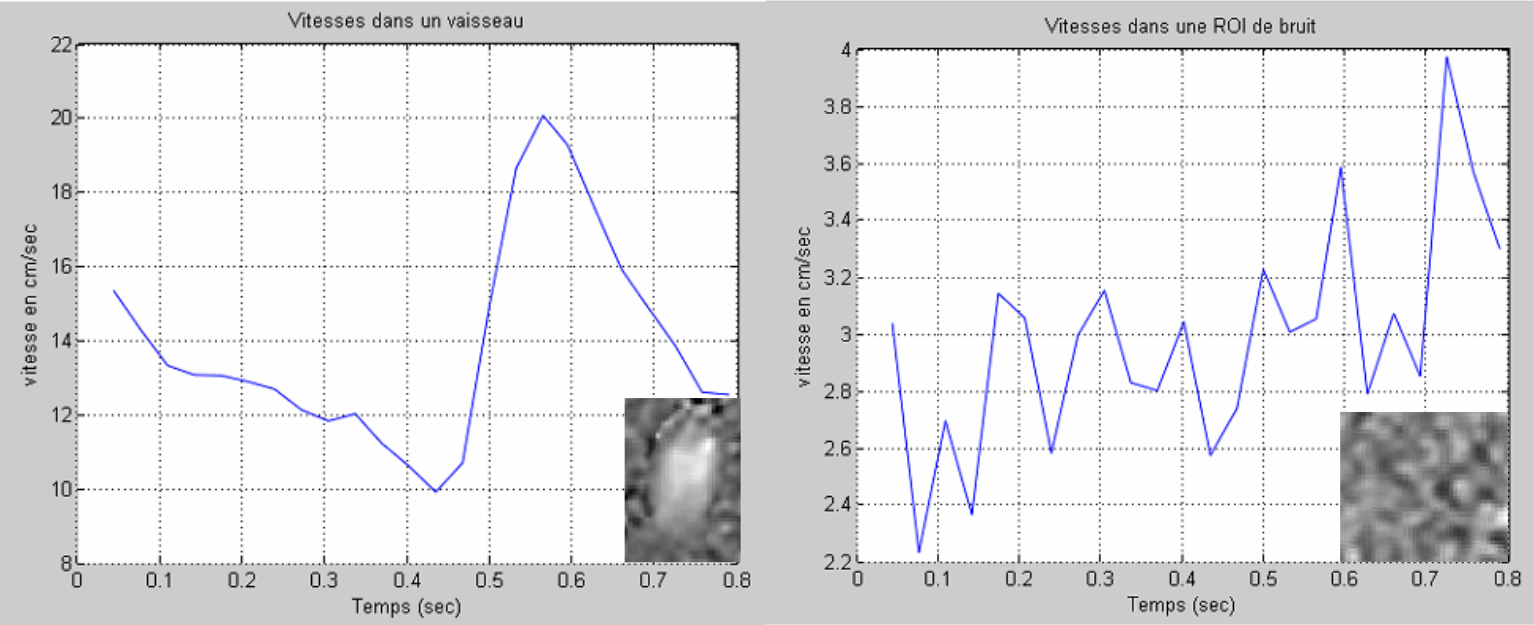
\includegraphics[width=14cm]{3_4_bruit_contraste_phase}
\caption{Différence de cinétique entre un vaisseau et du bruit en contraste de phase. A gauche les vitesses moyennes dans
le vaisseau, à droite dans le bruit.}
\label{fig:3_4_bruit_contraste_phase}	
\end{figure}
Les images en contraste de phase disposent d’une consistance temporelle au niveau du vaisseau,
c’est-à-dire qu’ensemble elles aboutissent à un signal 1D cohérent. Or le signal à l’extérieur des
vaisseaux représente un bruit incohérent (Figure \ref{fig:3_4_bruit_contraste_phase}). En effet, le LCS et le sang ont un mouvement
synchronisé sur le cycle cardiaque, et nous savons qu’une séquence est un échantillonnage d’un cycle
cardiaque, donc il est possible d’utiliser la dimension temporelle pour notre segmentation.

On notera tout d’abord les approches dites de « clustering » ou regroupement par similitude sur
la base de la cinétique du signal (\cite{Gaffney2004}). On recherche les courbes disposants d’une cinétique similaire à
une courbe de référence (pouvant par exemple être définie par l’utilisateur en indiquant un voxel dans
un vaisseau). Dans ces méthodes, il convient de définir des classes de similitudes. La séparation à
laquelle nous souhaiterions aboutir est une séparation en deux classes. Aucun système de clustering
simple de ne fournit une telle séparation qui soit satisfaisante au vu des données.

Par ailleurs, nous avons développé une méthode basée sur la transformée de Fourier. Les courbes
de vitesses sont obtenues à partir de valeurs discrètes : il y a une valeur par image, et chaque valeur
est séparée de la suivante par un intervalle de temps régulier qui est $\frac{T}{nb}$, avec $T$ la durée d’un cycle
cardiaque, et $nb$ le nombre d’images de la séquence. On utilise alors une transformée de Fourier
discrète. 
%%%
\begin{figure}[!b]
\centering
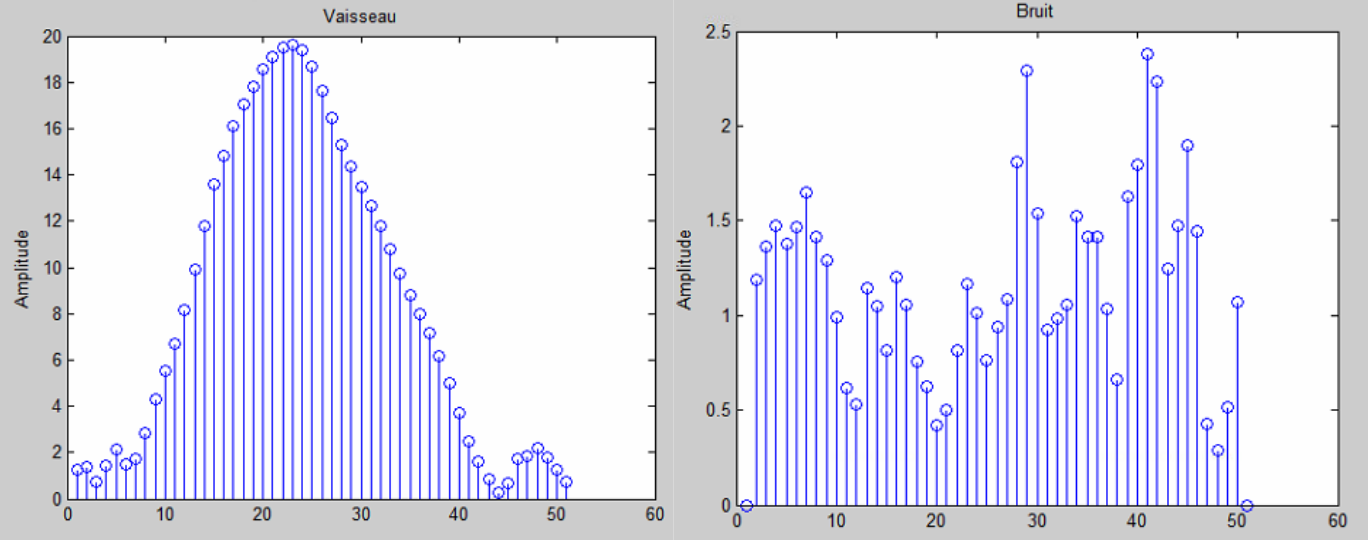
\includegraphics[width=14cm]{3_5_TF_sang_bruit}
\caption{Amplitude de la transformée de Fourier d’un signal au cours du temps pour un voxel de sang, et un voxel de bruit.
On remarque la différence d'échelle.}
\label{fig:3_5_TF_sang_bruit}	
\end{figure}
Si l’on observe la Figure~\ref{fig:3_5_TF_sang_bruit}, il est clair qu’il existe une différence entre un voxel contenant de
l’information (du sang ici) et un voxel de bruit. Le critère important à retenir ici est la valeur de
l’amplitude. On remarque en effet, qu’il existe un facteur dix au moins entre le bruit et le sang. Il est
donc possible de segmenter un vaisseau dans l’image sur simple seuillage sur la base de cette
amplitude. Ce seuil, défini automatiquement, peut être ajusté par l’utilisateur afin d’obtenir un résultat
satisfaisant (Figure~\ref{fig:3_6_segmentation_TF}).
%%%
\begin{figure}[!t]
\centering
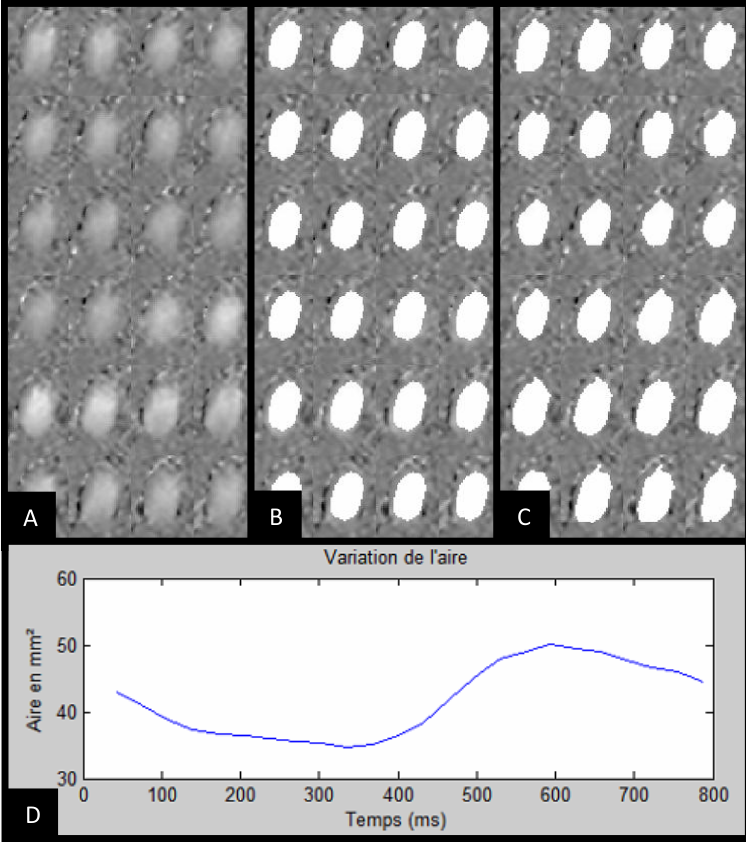
\includegraphics[width=14cm]{3_6_segmentation_TF}
\caption{Segmentation par la méthode basée sur la transformée de Fourier. A) la région d’intérêt au cours du temps avec
le vaisseau en son centre (ordre des images de gauche à droite et de haut en bas). B) La segmentation sur la base d’une
transformée de Fourier sur l’ensemble de la cinétique. C) Segmentation par transformée de Fourier sur une fenêtre glissante
(5 images). D) Evolution de l’aire obtenue par la méthode C.}
\label{fig:3_6_segmentation_TF}	
\end{figure}
Dans ces deux approches, la segmentation est unique pour toutes les images (pas d’évolution
d’aire). Pour pallier à ce problème, il sera nécessaire d’utiliser une fenêtre glissante. Considérons une image à un temps T, la segmentation du vaisseau à ce temps peut être
obtenue en prenant le signal du temps T-2 au temps T+2 (kernel 5 images). Cette fenêtre de recherche
de 5 images est ensuite décalée pour obtenir la segmentation à T+1. Sur la base de 5 images il devient
très difficile de discriminer deux classes dans l’approche « clustering ». En revanche, le critère de la
méthode de transformée de Fourier se révèle suffisamment robuste pour discriminer facilement le
bruit du signal d’intérêt sur la base de ce petit nombre d’images. Le résultat de cette méthode est
donné dans la Figure~\ref{fig:3_6_segmentation_TF} C et D où l’on montre que l’estimation de l’évolution de l’aire du vaisseau au cours du temps est conforme à ce qui est attendu.


%%%
\begin{figure}[!t]
\centering
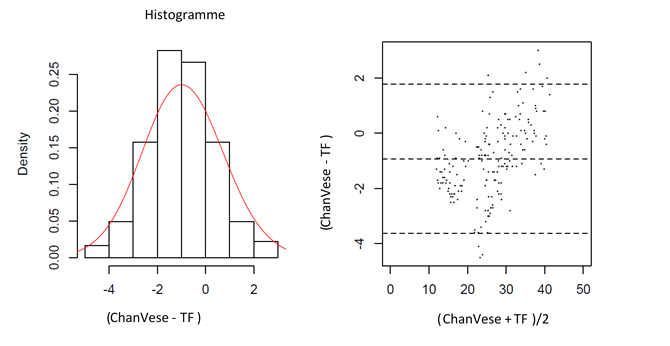
\includegraphics[width=14cm]{PCMRi_TF_CHANVESE}
\caption{Graphiques de Bland-Altman comparant les vitesses mesurées via une segmentation Chan-Vese et par transformée de Fourier (TF). L'histogramme représente la répartition de la différence entre les deux méthodes.}
\label{fig:PCMRi_TF_CHANVESE}	
\end{figure}

%%%
\begin{figure}[!t]
\centering
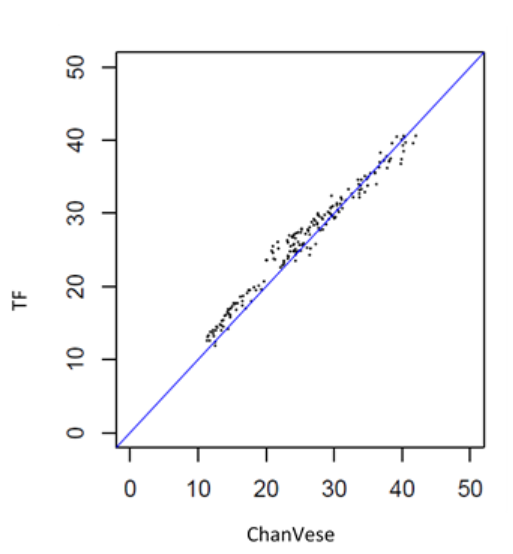
\includegraphics[width=10cm]{PCMRi_TF_CHANVESE_concordance}
\caption{Analyse de concordance entre les vitesses mesurées via une segmentation Chan-Vese et par transformée de Fourier (TF).}
\label{fig:PCMRi_TF_CHANVESE_concordance}	
\end{figure}

Notre méthode a été comparée avec une approche standard de type Chan-Vese (\cite{Chan2001}) en collaboration avec le docteur Eker Omer. Cette approche est de type contour actif, elle consiste à partir d'un masque initial à trouver une segmentation en développant les contours de l'objet. Dans nos essais, 8 patients ou volontaires ont réalisé des acquisitions IRM en contraste de phase. Au total 182 mesures de vitesses et débits ont été réalisées. La comparaison des deux méthodes sur la mesure de la vitesse a été réalisée via un Bland-Altman (Figure~\ref{fig:PCMRi_TF_CHANVESE}). On remarque que notre méthode a tendance à fournir des vitesses légèrement plus élevées que l'approche de Chan-Vese. Ceci s'explique par l'approche différente de segmentation. En effet, l'algorithme de Chan-Vese fonctionne sur les images de magnitudes et se sert ainsi du contraste structurel. Notre approche en revanche se base uniquement sur la cinétique du signal. Notre approche aura ainsi tendance à segmenter de façon plus nette le sang uniquement, tandis que le Chan-Vese aura tendance à prendre une surface légèrement plus importante. Les résultats de la Figure~\ref{PCMRi_TF_CHANVESE_concordance} montrent une très bonne concordance des deux méthodes avec un nuage de points se situant sur la ligne à 45°. Il semble ainsi que notre méthode permet de mesurer correctement les vitesses. Gardons à l'esprit malgré tout que la mesure est moins fiable dans le cadre de pathologies ou d'anévrysmes.
%%%
%%%
\subsection{Perfusion : imagerie par marquage des protons du sang artériel (ASL)}
Les techniques de mesure de la perfusion cérébrale impliquent pour la plupart l’injection d’un
produit de contraste (Dynamic contrast-enhanced, Dynamic Susceptibility Contrast,~\cite{Calamante2010},~\cite{OConnor2011}),
déconseillée pour certaines populations à risques (femmes enceintes, personnes âgés). Les techniques
de marquage des protons artériels du sang ou « Arterial Spin Labeling » (ASL) au contraire, permettent
une exploration non invasive de la perfusion cérébrale en utilisant un traceur endogène : les protons
du sang artériel eux même, marqués magnétiquement. Il s’agit d’une technique qui repose sur
l’acquisition de deux volumes, l’un avec marquage des protons artériels et l’autre sans marquage
(contrôle). Le marquage est réalisé au niveau du cou à l’aide d’une impulsion radiofréquence à 180°,
dite impulsion d’inversion. Par la suite le sang évolue vers les niveaux supérieurs via les artères,
artérioles puis capillaires, pour arriver dans la zone à imager. Après un temps $TI$ (temps d’inversion),
l’acquisition des images est réalisée via un technique d’imagerie rapide (Figure~\ref{fig:3_7_ASL}). 
%%%
\begin{figure}[!t]
\centering
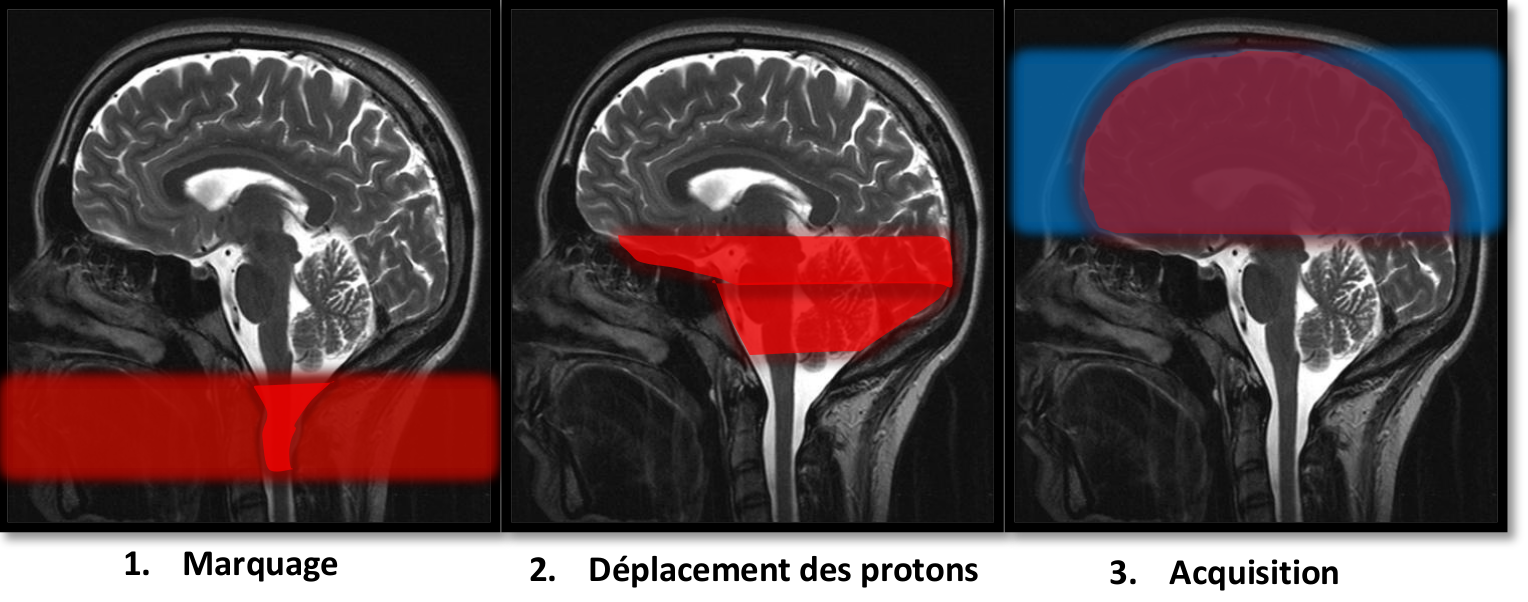
\includegraphics[width=14cm]{3_7_ASL}
\caption{Principe de base de l'acquisition ASL. La zone de marquage est en orange, le sang marqué en rouge, et la zone à
imager en bleu.}
\label{fig:3_7_ASL}	
\end{figure}
Du fait de
l’inversion, le sang marqué disposera d’un signal plus faible que le sang non marqué.

Une acquisition sans inversion est par la suite réalisée. La soustraction de l’image marquée à
l’image contrôle permet d’éliminer la contribution des tissus statiques afin de ne conserver que
l’information relative à la perfusion (Figure~\ref{fig:3_8_principe_debit_ASL}).
%%%
\begin{figure}[!t]
\centering
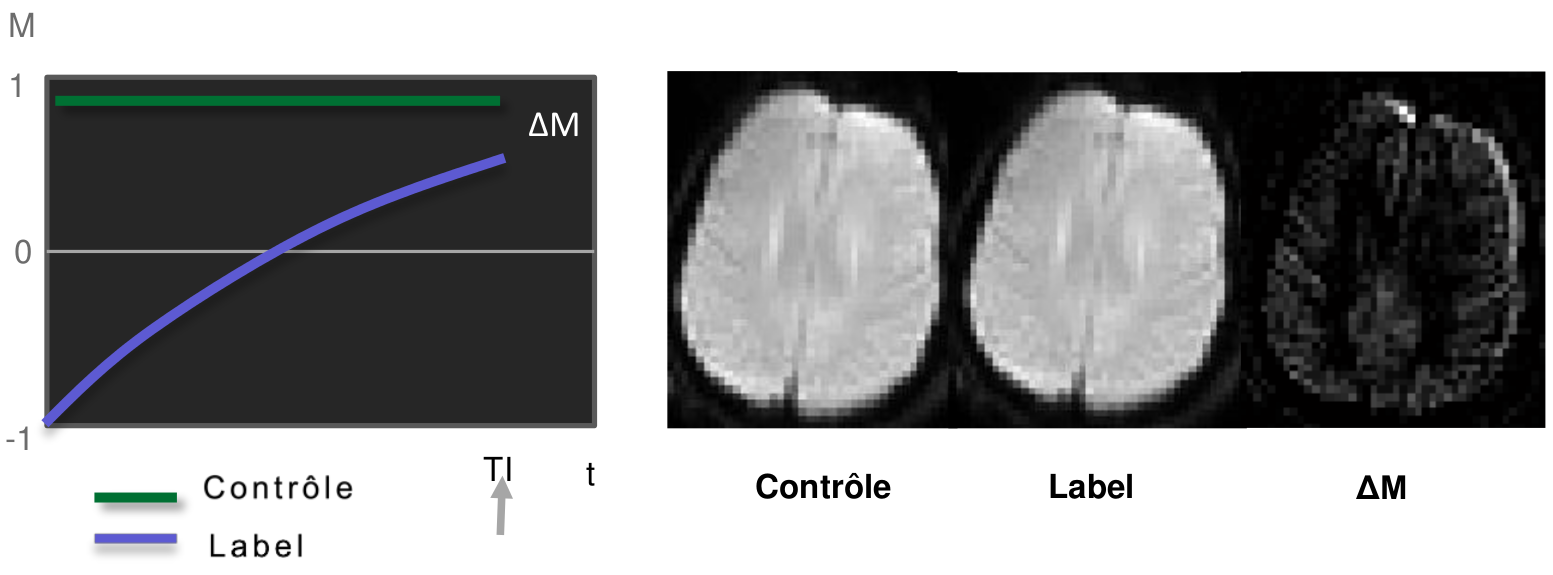
\includegraphics[width=14cm]{3_8_principe_debit_ASL}
\caption{Principe de la mesure de débit en ASL. A gauche, l’évolution de la magnétisation ($M$) pour l’image contrôle (vert) et
l’image marquée (bleu) au court du temps ($t$) après l’impulsion radiofréquence. L’acquisition est réalisée après le temps $TI$, la
différence $\Delta M$ étant directement proportionnel au débit. A droite les images contrôle, marquée (label) et la différence ($\Delta M$),proportionnel au débit.}
\label{fig:3_8_principe_debit_ASL}	
\end{figure}
L’image de la différence $\Delta M$ est donc directement proportionnelle au débit perfusionnel : on
parle d’image pondérée en perfusion. Cependant cette différence n’est que de l’ordre de quelques
pourcents. Pour obtenir un rapport signal sur bruit (RSB) satisfaisant il est donc nécessaire de répéter
ces acquisitions plusieurs dizaines de fois puis de les moyenner. Le passage d’une donnée purement
qualitative (pondération en perfusion) à une information quantitative (débit en ml/100g/min) requiert
ensuite l’application d’un modèle.

Plusieurs méthodes d’acquisitions existent selon le mode de marquage des protons. Nous
distinguerons ainsi les séquences pulsées (PASL) et les séquences pseudo-continues (pCASL). La
séquence pulsée telle qu’elle est implémentée à l’heure actuelle offre des temps d’acquisition court
autorisant l’utilisation du multi-$TI$ (temps d’inversion) dans le but d’affiner l’estimation du débit. La
séquence pseudo-continue, elle, fournit un meilleur rapport signal sur bruit mais en un temps pouvant
être plus long. Le détail de ces acquisitions sera développé dans un chapitre dédié à l’ASL (Chapitre~\ref{chap:asl}).
%%%
%%%
%%%
\section{Le protocole complet d'acquisition}
\label{sec:protocole}
Aux séquences adaptées à l’imagerie morphologique nous ajoutons deux séquences qui nous
donnent accès aux éléments dynamiques :
\begin{itemize}
\item une imagerie dynamique en contraste de phase afin d’obtenir le flux dans le sinus sagittal
supérieur, l’artère basilaire, et les carotides internes, paramètres : champ de vue 14 x 14
cm, temps d’écho = 10.48 ms, temps de répétition = 32.36 ms, angle de bascule = 15°,
taille de voxel = 0.31 x 0.31 x 3.1 mm$^3$, vitesse d’encodage 80 cm/s (artères) et 50 cm/s
(veines).
\item une imagerie ASL permettant de quantifier la perfusion. Ces séquences évoluant
rapidement il conviendra à l’utilisateur de choisir celle qui fournit les meilleurs résultats.
Nous proposons d’utiliser une ASL pulsée 3D FAIR-Q2TIPS (\cite{Gunther2005}) multi-$TI$ lorsque le sujet
présente une pathologie pouvant affecter fortement le temps de transit (incertitude sur le
temps d’inversion optimal), 16 temps d’inversion de 480 à 4080 ms, durée du bolus 700
ms, champ de vue = 13.4 x 13.4 cm, temps d’écho = 14.94 ms, temps de répétition = 3500
ms, taille du voxel = 3 x 3 x 3 mm$^3$; ou une ASL pseudo-continue 3D simple $TI$ (\cite{Wu2007}) lorsque
le sujet est bien caractérisé : temps d’inversion = 3000 ms, durée du bolus = 1500 ms,
champ de vue = 12.6 x 12.8 cm, temps d’écho = 15.62 ms, temps de répétition = 4600 ms,
taille du voxel = 1.5 x 1.5 x 3 mm$^3$, 42 coupes. Le détail de ces techniques est décrit dans le
chapitre~\ref{chap:asl}. Notons que l'intégralité du traitement de cette imagerie est réalisé par des codes implémentés dans le cadre de notre travail. Parmis les traitement on évoquera la correction de mouvement, la quantification, la correction d'effets de volumes partiels etc.
\end{itemize}
L’ensemble constitue un protocole de 45 minutes.




	
\bibliography{jeremythesebib}{}
\bibliographystyle{francaissc}